%%%%%%%%%%%%%%%%%%%%%%%%%%%%%%%%%%%%%%%%%%%%%%%%%%%%%%%%%%%%%%%%%%%%%
% LaTeX Template: Project Titlepage Modified (v 0.1) by rcx
%
% Original Source: http://www.howtotex.com
% Date: February 2014
% 
% This is a title page template which be used for articles & reports.
% 
% This is the modified version of the original Latex template from
% aforementioned website.
% 
%%%%%%%%%%%%%%%%%%%%%%%%%%%%%%%%%%%%%%%%%%%%%%%%%%%%%%%%%%%%%%%%%%%%%%

\documentclass[12pt]{report}
\usepackage[a4paper]{geometry}
\usepackage[myheadings]{fullpage}
\usepackage{fancyhdr}
\usepackage{lastpage}
\usepackage{graphicx, wrapfig, subcaption, setspace, booktabs}
\usepackage[T1]{fontenc}
\usepackage[font=small, labelfont=bf]{caption}
\usepackage{fourier}
\usepackage[protrusion=true, expansion=true]{microtype}
\usepackage[english]{babel}
\usepackage{sectsty}
%\usepackage{url, lipsum}
\usepackage{color}

\definecolor{dkgreen}{rgb}{0,0.6,0}
\definecolor{gray}{rgb}{0.5,0.5,0.5}
\definecolor{mauve}{rgb}{0.58,0,0.82}
\usepackage{mathtools}
\usepackage{wallpaper}
\usepackage{amsmath}
\usepackage{amssymb}
\usepackage{url}
\usepackage{listings}
\lstset{language=Python,
	aboveskip=3mm,
	belowskip=3mm,
	showstringspaces=false,
	columns=flexible,
	basicstyle={\small\ttfamily},
	numbers=none,
	numberstyle=\tiny\color{gray},
	keywordstyle=\color{blue},
	commentstyle=\color{dkgreen},
	stringstyle=\color{mauve},
	breaklines=true,
	breakatwhitespace=true,
	tabsize=3
}


\newcommand{\HRule}[1]{\rule{\linewidth}{#1}}
\onehalfspacing
\setcounter{tocdepth}{5}
\setcounter{secnumdepth}{5}

%-------------------------------------------------------------------------------
% HEADER & FOOTER
%-------------------------------------------------------------------------------
\pagestyle{fancy}
\fancyhf{}
\setlength\headheight{15pt}
%\fancyhead[L]{Student ID: 1034511}
%\fancyhead[R]{Anglia Ruskin University}
\fancyfoot[R]{Page \thepage\ of \pageref{LastPage}}
%-------------------------------------------------------------------------------
% TITLE PAGE
%-------------------------------------------------------------------------------

\begin{document}

\title{ \normalsize \textsc{}
		\\ [2.0cm]
		\HRule{0.5pt} \\
		\LARGE \textbf{A comparative study of Word2Vec word embeddings}
		\HRule{2pt} \\ [0.5cm]
		\normalsize \today \vspace*{5\baselineskip}}

\date{}

\author{
	    Misikir Eyob Gebrehiwot\\
		ID: 336114 \\ 
	}
%\ThisCenterWallPaper{0.5}{language}
%\ThisURCornerWallPaper{0.25}{language}
\maketitle
%\tableofcontents
\newpage

%-------------------------------------------------------------------------------
% Section title formatting
\sectionfont{\scshape}
%-------------------------------------------------------------------------------

%-------------------------------------------------------------------------------
% BODY
%-------------------------------------------------------------------------------

\section*{1. Introduction}
Representation of words as vectors in a high dimensional vector space is a vital
step of the state-of-the-art natural language processing techniques, which employ
advanced matrix computations to gain insight into semantic and syntactic similarities
between words and/or documents. The two main language models in this regard are 
\emph{context-counting} and \emph{context-predicting} models.

Context-counting models construct a word co-occurrence matrix from a context window
in a given corpus. The underlying assumption is that similar words will appear in the same context, and hence their vector representations will be closer to each other. However, the size of raw co-occurrence matrices grows exponentially with the vocabulary. For this and other performance reasons, dimensionality reduction techniques such as \emph{Latent Semantic Indexing} are often used in context-counting models together with \emph{Weighting} techniques \cite{Manning:1999:FSN:311445,ARIS:ARIS1440380105}.

On the other hand, context-predicting models approach the word embedding problem as a supervised learning task, which tries to predict the vector embedding of a target word directly from the context. That is, given the embedding of other words in the context it 
learns the embedding of the target word (or vise versa) \cite{Bengio:2003:NPL:944919.944966,mikolov2013efficient}. Baroni et al. conducted an extensive comparison between count and predictive models in \cite{marcobaroni2014predict} 
and reported that the predictive models performed significantly better than the count models in a number of evaluation tasks.

Bengio et al. proposed one of the first predictive models, which is a \emph{feedforward Neural Network Language Model (NNLM)} \cite{Bengio:2003:NPL:944919.944966}. The end result 
of an NNLM is to learn a probability distribution for words given other words in a context.
Architecturally, it has four layers. The first layer is an input layer where N previous words of a context are encoded using one-hot encoding. Layer 2: Is a projection layer where each word in the vocabulary is represented in a high dimensional space. This is a dense representation of the input, where each of the $N$ context words are represented by a $D$-dimensional vector. That is, this layer produces an $N\times D$ matrix.
Layer 3 is a hidden layer in a normal neural network. If the hidden layer has $H$ nodes, there will be $H\times N$ matrix of weights. Layer 4 is the output layer of the neural network. At this layer, probability is assigned to each word in the vocabulary.

More recently, Mikolov et al. proposed a simple but yet efficient neural network model \cite{mikolov2013efficient}, which is implemented as the \emph{Word2Vec toolkit\footnote{https://code.google.com/archive/p/word2vec/}}. In contrast to \emph{NNLM  Word2Vec} does not use the hidden layer. For a clear and illustrative 
explanation of the Word2Vec toolkit see \cite{rong2014word2vec}. In the following section, we will discuss the two main architectures and parameter settings in Word2Vec.

In this work, we explore the different parameter settings in Word2Vec and their effect in 
model training time and accuracy using a preprocessed Wikipedia (English) text corpus. Additionally, a model pre-trained on the Google news data set is also used\footnote{https://drive.google.com/file/d/0B7XkCwpI5KDYNlNUTTlSS21pQmM/edit}.

\section*{2. Word2Vec architectures and parameters}
There are two distinct architecture choices in Word2Vec: \emph{Continuous Bag of Words (CBOW)} and \emph{Skip-gram}. In a CBOW model, the objective is to predict the current word
given the context from words in the history. On the other hand, Skip-gram predicts the words within a context window given the current word. 

In addition to architecture, some parameter choices also impact the training time and/or accuracy of a Word2Vec model. The main parameters are discussed below.

\noindent \textbf{\emph{Training algorithm.}} The training algorithm can be \emph{hierarchical softmax}
or \emph{negative sampling}. Hierarchical softmax attempts to maximize the log-likelihood of a target word, whereas negative sampling minimizes the log-likelihood of negative samples.

\noindent \textbf{\emph{Window size.}} This is the context window size. That is, the maximum number of words to take into context when predicting the current word (CBOW) or the maximum number of predictions to make per word (Skip-gram).

\noindent \textbf{\emph{Down sampling.}} A probability for randomly discarding frequent words
aimed to reduce the imbalance between most common and rare words.

\noindent \textbf{\emph{Size.}} This is the number of feature vectors used to represent words, that is the dimensionality of vector space.

\section*{3. Methods}
To evaluate the performance of the new and pre-trained word embeddings, three evaluation methods are applied using data provided in the course folder.

\noindent \textbf{\emph{The nearest neighbors evaluation task.}} This method is useful in testing the syntactic and semantic similarity of word vectors and their nearest neighbors using (cosine) distance
as a measure. However, the evaluation is limited to a subjective qualitative study. Although all the models are tested using all the words in this set, only a subset of the results are discussed in this report.

\noindent \textbf{\emph{The analogical reasoning evaluation task.}} This task set, originally from \cite{mikolov2013efficient}, tests the ability of a model to identify analogies such as 
\emph{If Paris is to France, Helsinki is to \underline{\textcolor{white}{aljdlfj}}}. Out of the available fourteen categories of analogical tests, the following five sets are
used in this project:
\begin{itemize}
	\item \emph{Capital-world.} Similar to the example given above, this set tests whether the model can correctly make an analogy between countries in the world and their capitals. 
	\item \emph{City-in-state.} This set contains analogies between
	states and their cities in the United States. 
	\item \emph{Currency.} This set evaluates a model on financial analogies like \emph{United States is to Dollar, Finland is to \underline{\textcolor{white}{aljdlfj}}}
	\item \emph{Family.}  This set evaluates a model on family analogies like \emph{boy is to girl, brother is to \underline{\textcolor{white}{aljdlfj}}}
	\item \emph{Opposite.} This set evaluates whether a model is able to correctly identify the opposite of a given word by analogy. The test phrases are similar to: \emph{clear is to unclear, efficient is to \underline{\textcolor{white}{aljdlfj}}}.
		
\end{itemize}

\noindent\textbf{\emph{The concrete noun categorization task.}} This evaluation set contains a list of $44$ concrete nouns and their categories in three levels. In the first level, each noun is categorized into two groups: \emph{"natural"} or \emph{"artifact."} The second level further categorizes the words into three groups: \emph{"animal","vegetable", \emph{and} "artifact"}. The last level is the most detailed of all, and categorizes the nouns into six groups: \emph{"bird","groundAnimal", "fruitTree", "green", "tool" \emph{and} "vehicle."}
For this task, the word vectors of all $44$ words are used in a K-means clustering algorithm\footnote{http://scikit-learn.org/stable/modules/clustering.html\#k-means} by setting the number of clusters to $2$, $3$, and $6$ corresponding to the three levels discussed above. The classification error is calculated by
\[
\text{error} = \frac{C(\text{misclassified words})}{C(\text{words})},
\] 
\noindent where the numerator is the count of misclassified words and the denominator is the total number of words (=$44$). Accuracy of the model is then $(1-error)\times 100\%$. Here the performance of K-means clustering also impacts the performance of the model under study. However, the goal of this project is to study the impact of 
parameter values in the performance of Word2Vec models. Thus, the assumption is that the effect of K-means on the performance of a model is uniform across different parameter settings.


\section*{4. Experiments}
The main goal of this project is to evaluate the performance of Word2Vec models. To this end, two approaches are used. First, the performance of a pre-trained word embedding is evaluated. Second, we train a Word2Vec model by 
selecting a number of parameter values. For this part, we selected the following parameters and chose two values 
per each parameter:

\begin{itemize}
	\item \textbf{Architecture:} CBOW and Skip-gram
	\item \textbf{Window size:} $\{5, 10\}$
	\item \textbf{Down sampling:} $\{0.001, 0.00001\}$
	\item \textbf{Feature vectors:} $\{200, 400\}$
\end{itemize}

\noindent So, a total of $16$ models are trained and their performance, both in terms of training time and accuracy, is studied. The experiment is conducted on a computer with a 4 core Intel Xeon (R) E5345 CPU and 6 GB of RAM running on Ubuntu 16.04.

\section*{5. Results}

\subsection*{5.1 Pre-trained model}
In this section, the performance of a pre-trained word embedding is discussed. The model was trained on part of Google News dataset, and contains 300-dimensional vectors for 3 million words and phrases. 
\begin{figure}
	\centering
	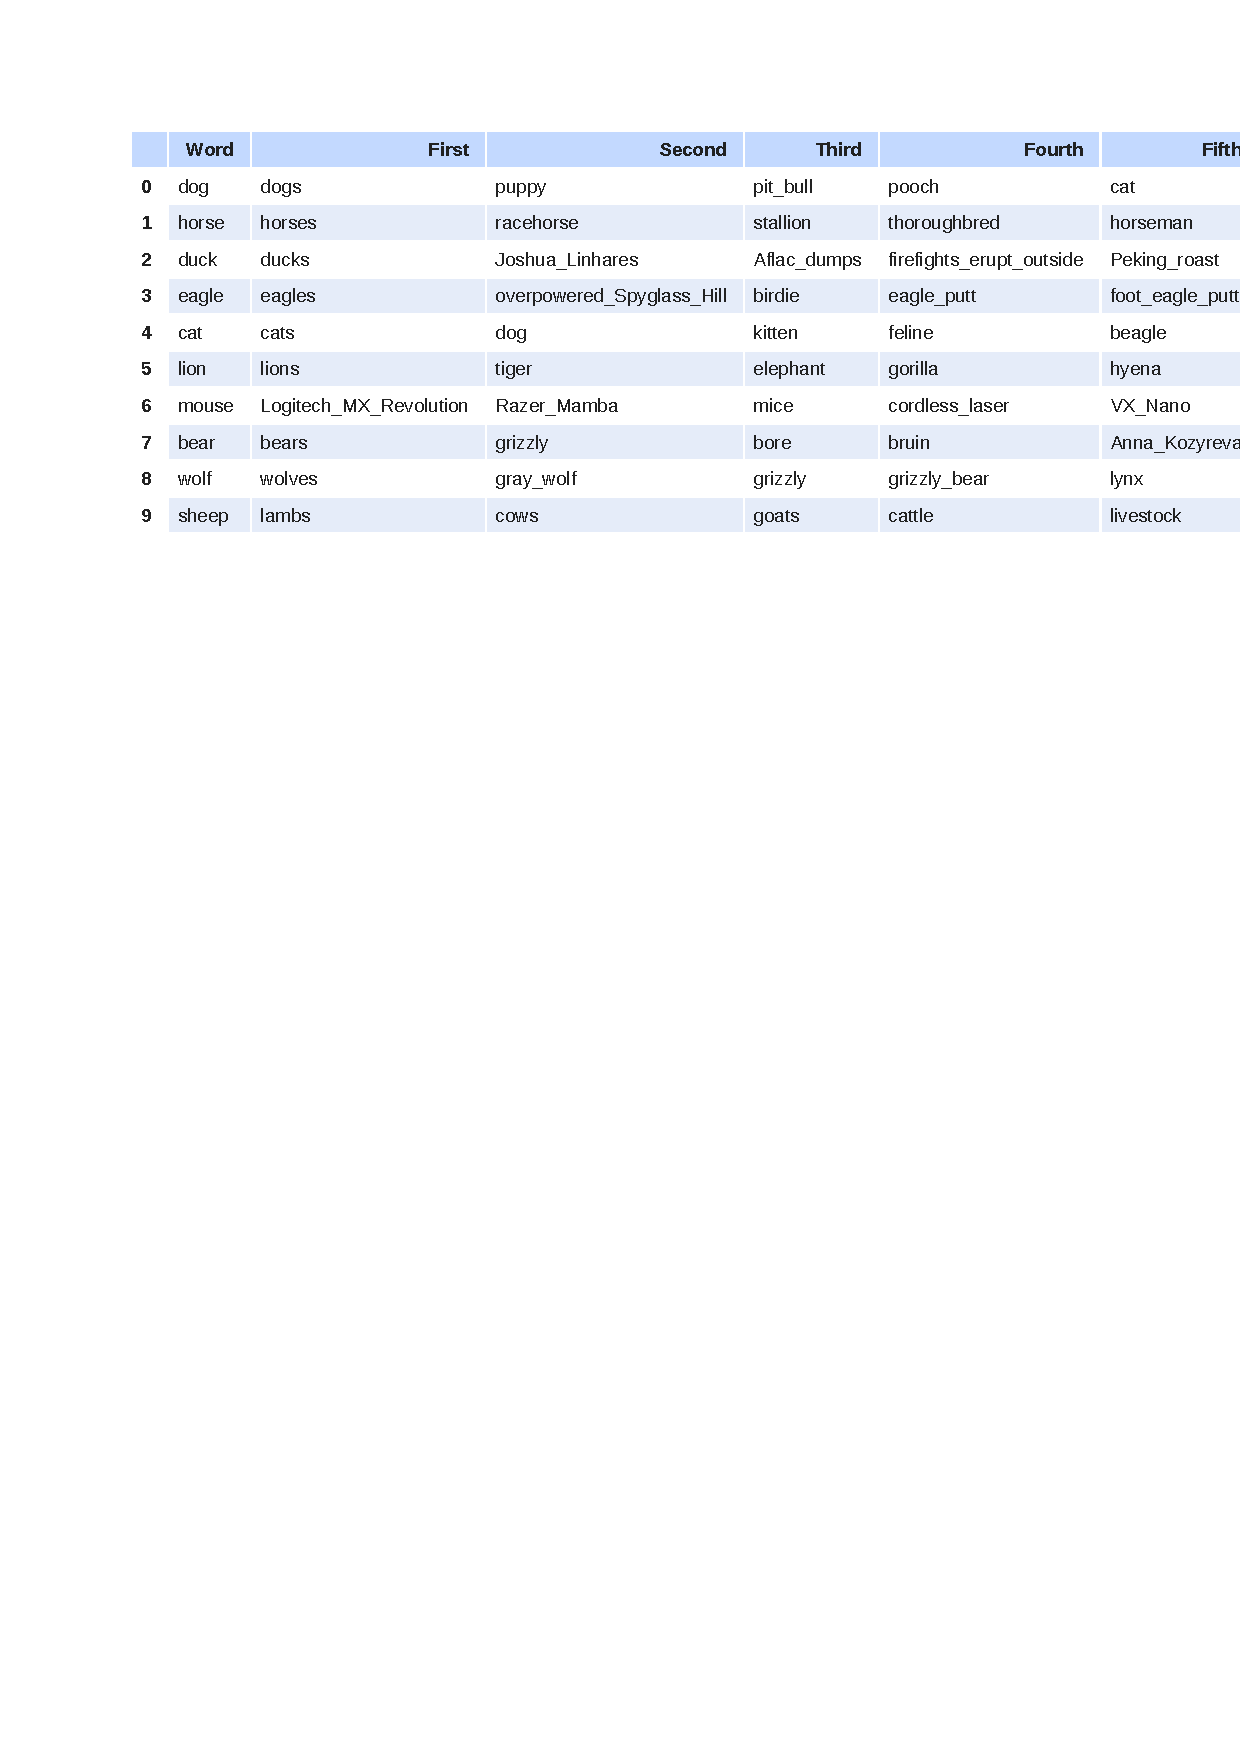
\includegraphics[trim=1cm 20cm 0cm 2cm, clip=true,width=\textwidth]{./Figures/google.pdf}
	\caption*{Table 1. Top 5 nearest words (labeled "First" to "Fifth") for the first ten words in the nearest neigbors evaluation set.}
	\label{fig:power}
	
\end{figure}

\begin{figure}
	\centering
	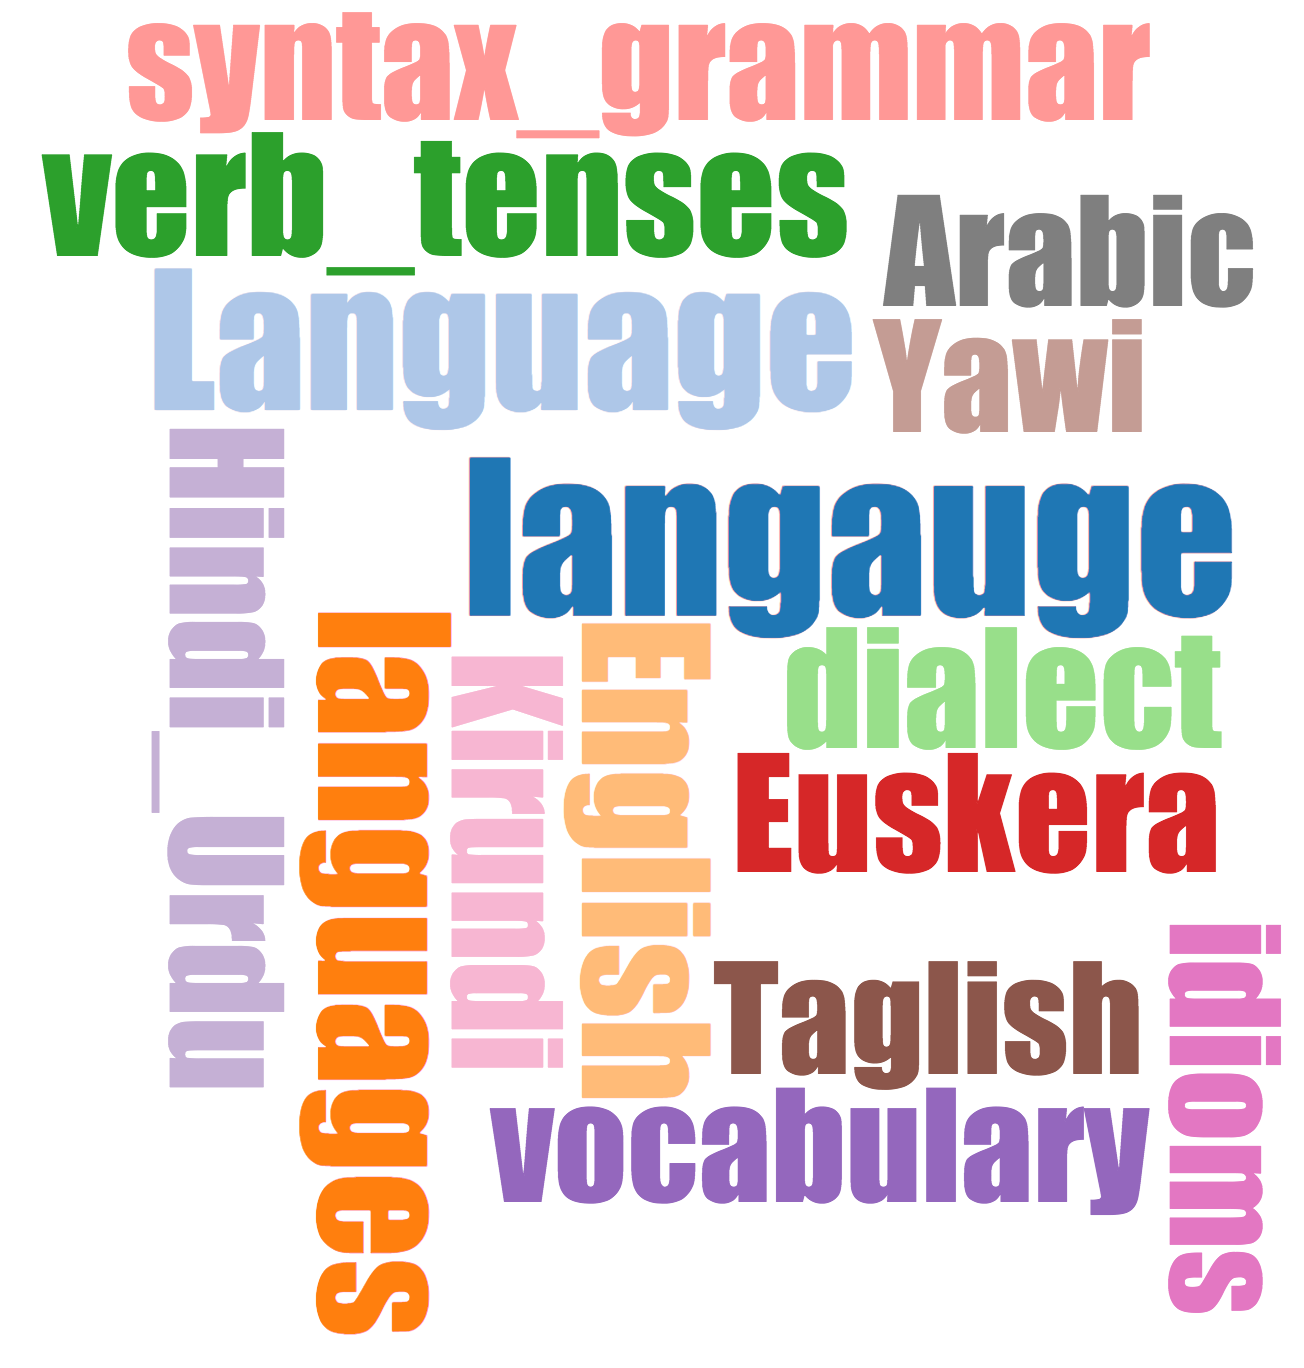
\includegraphics[trim=0.cm 0cm 0cm 0cm, clip=true,width=0.5\textwidth]{./Figures/language}
	\caption*{Figure 1. Top 15 nearest words to the word "language".}
	\label{fig:wordCloud}
\end{figure}	
	
\noindent\textbf{\emph{Nearest neighbors.}}  Table 1 shows the top five nearest words for the first ten words in the nearest neighbor evaluation set. The model was able to capture both syntactic (cat -- cats) and semantic (dog -- puppy) similarities between words. A word cloud visualization of the top 15 nearest words to the word "language" is depicted in Figure 1. Expected results such as "English" and "Arabic" are returned by the model. But the more interesting and unexpected word is "langauge". As the model was trained on a news data set, this result discloses the fact that "language" is often misspelled as "langauge". 

	\begin{figure}
		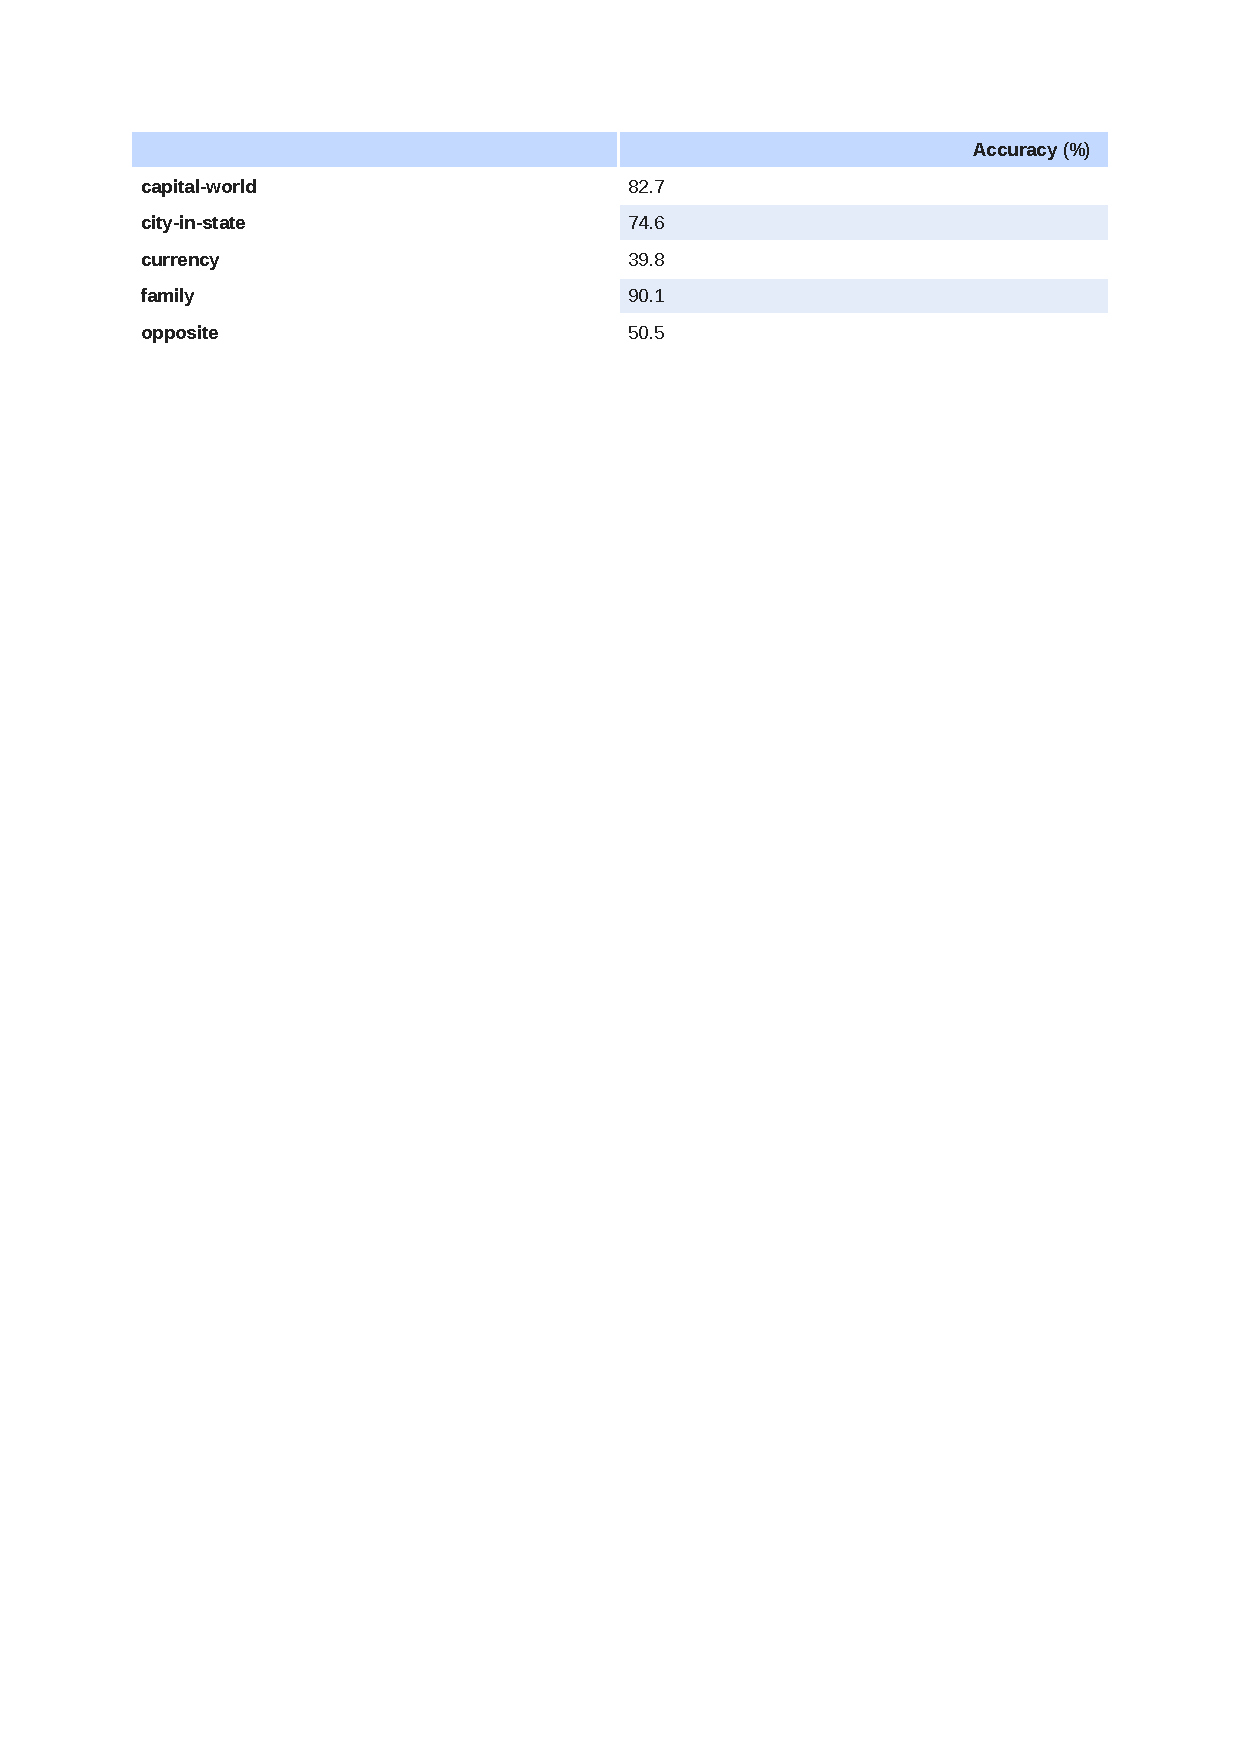
\includegraphics[trim=1.0cm 23cm 2cm 2cm, clip=true,width=0.9\textwidth]{./Figures/google-ana.pdf}
		\caption*{Table 2. Analogical reasoning task performance}
		\label{fig:analogical}
	\end{figure}

	\begin{figure}
		\centering
		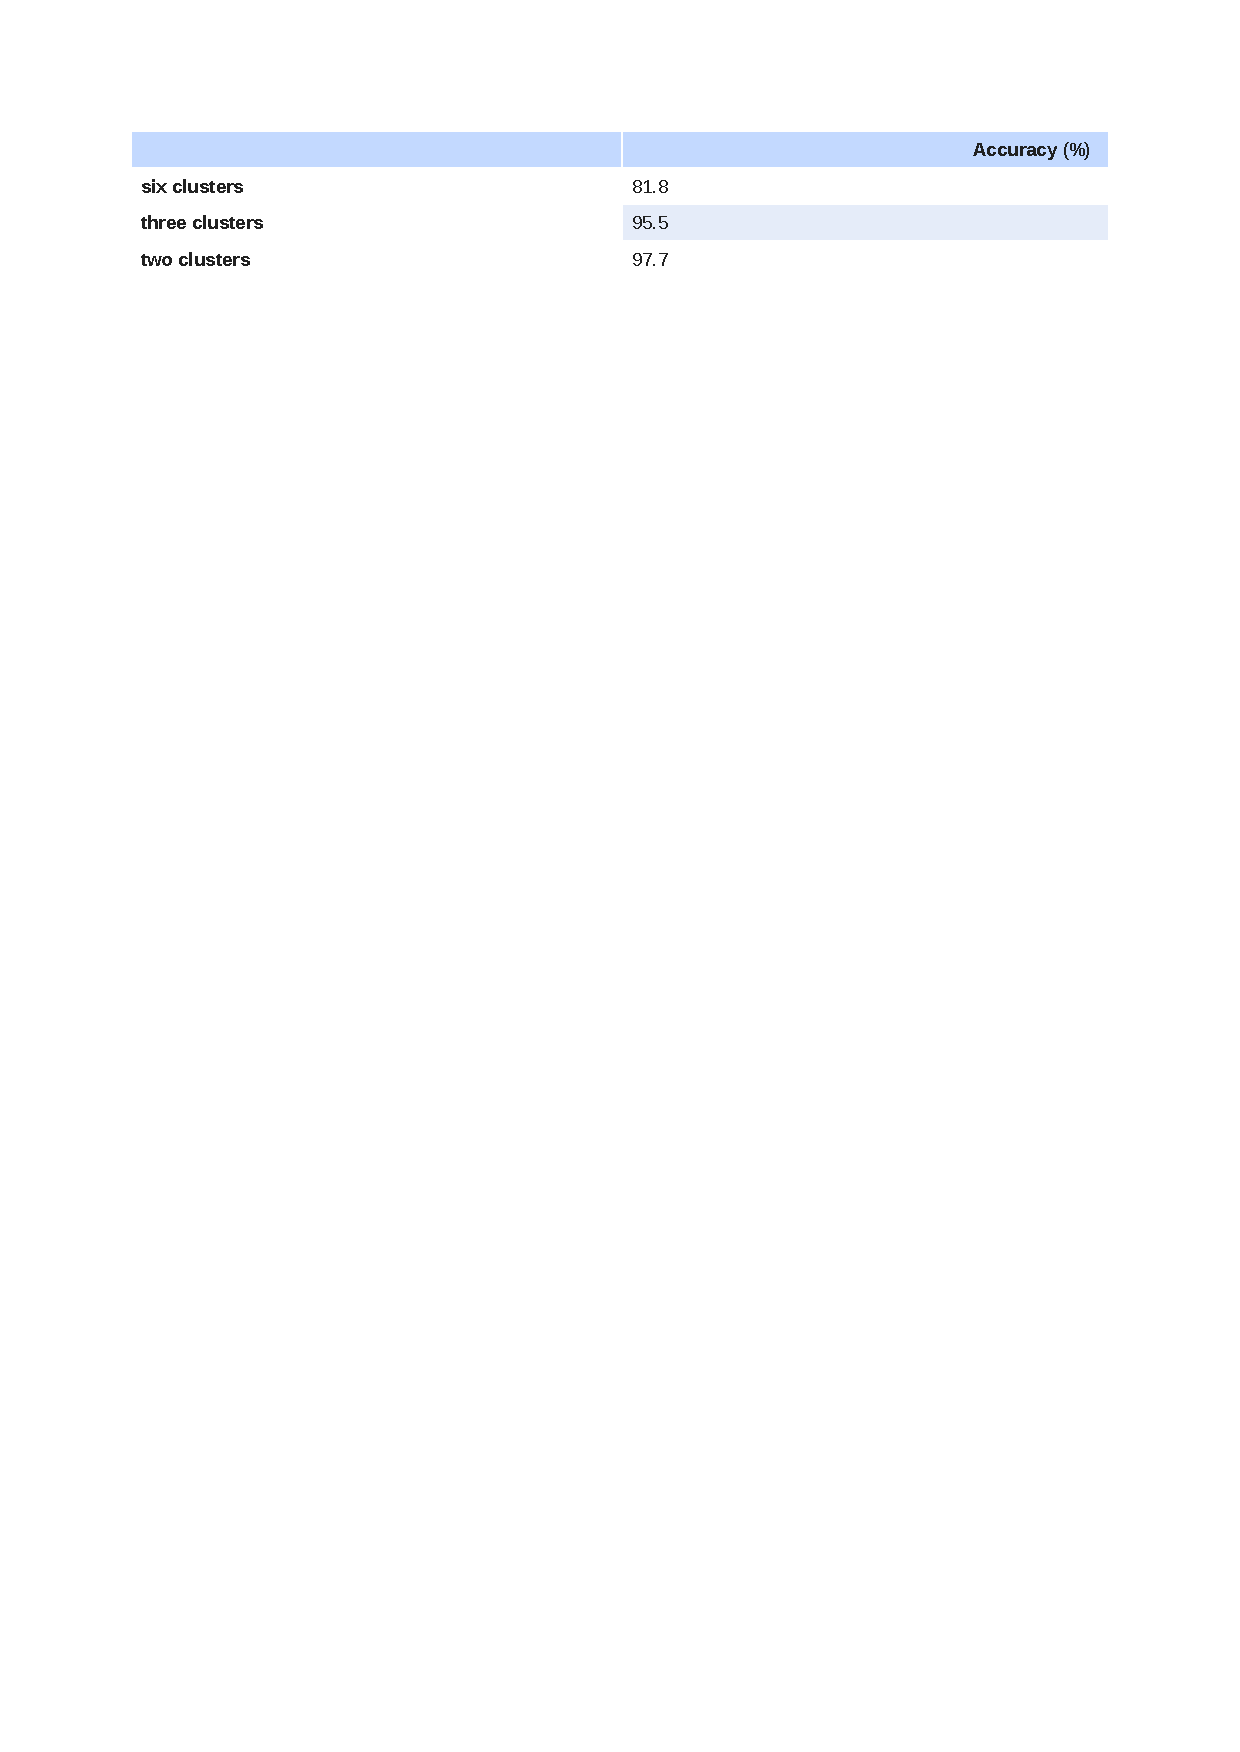
\includegraphics[trim=2.0cm 25cm 2cm 2cm, clip=true,width=0.9\textwidth]{./Figures/google-cluster.pdf}
		\caption*{Table 3. Concrete noun classification task performance}
		\label{fig:class}
	\end{figure}

\noindent\textbf{\emph{Analogical reasoning task.}} This evaluation is based on the five analogical reasoning evaluation sets, namely: the \emph{Capital-world, City-in-state, Currency, Family, and Opposite} sets. Word2Vec comes with a built-in 

\noindent\emph{"accuracy"} function that runs such analogical evaluations and returns a JSON-like data structure of correct and incorrect analogies returned by the model.
From this, a single accuracy percentage can be reported using 
\[
\text{accuracy} = 100 \times \frac{\text{correct analogies}}{\text{Total analogies}},
\]
\noindent see \cite{accuracy} for more on this. These numbers are given in Table 2 for the five analogy task sets. The model performed poorly on the \emph{Currency} set, which maybe due to
the lack of financial topics in the training data.

\begin{figure*}
	\centering
	\begin{subfigure}[b]{0.49\textwidth}
		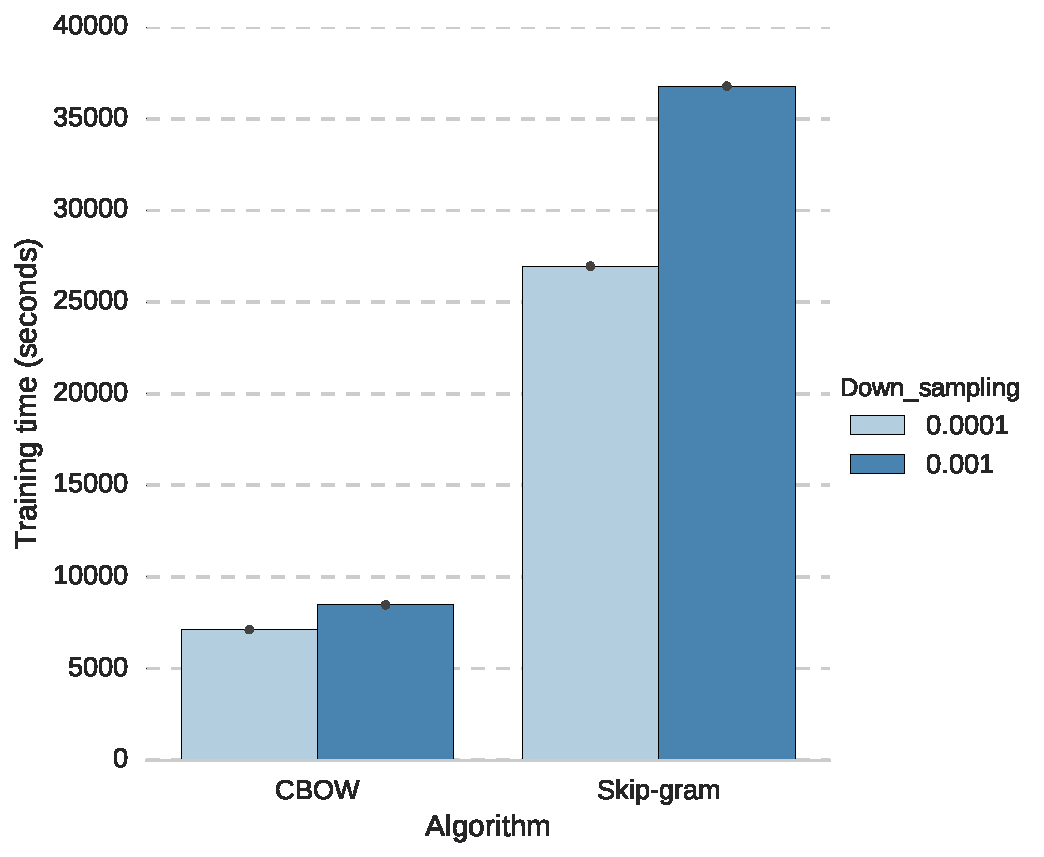
\includegraphics[width=0.9\textwidth]{./Figures/TrainTime-Down_sampling.pdf}
		\caption{}
		\label{fig:ws}
	\end{subfigure}
	\begin{subfigure}[b]{0.49\textwidth}
		\centering
		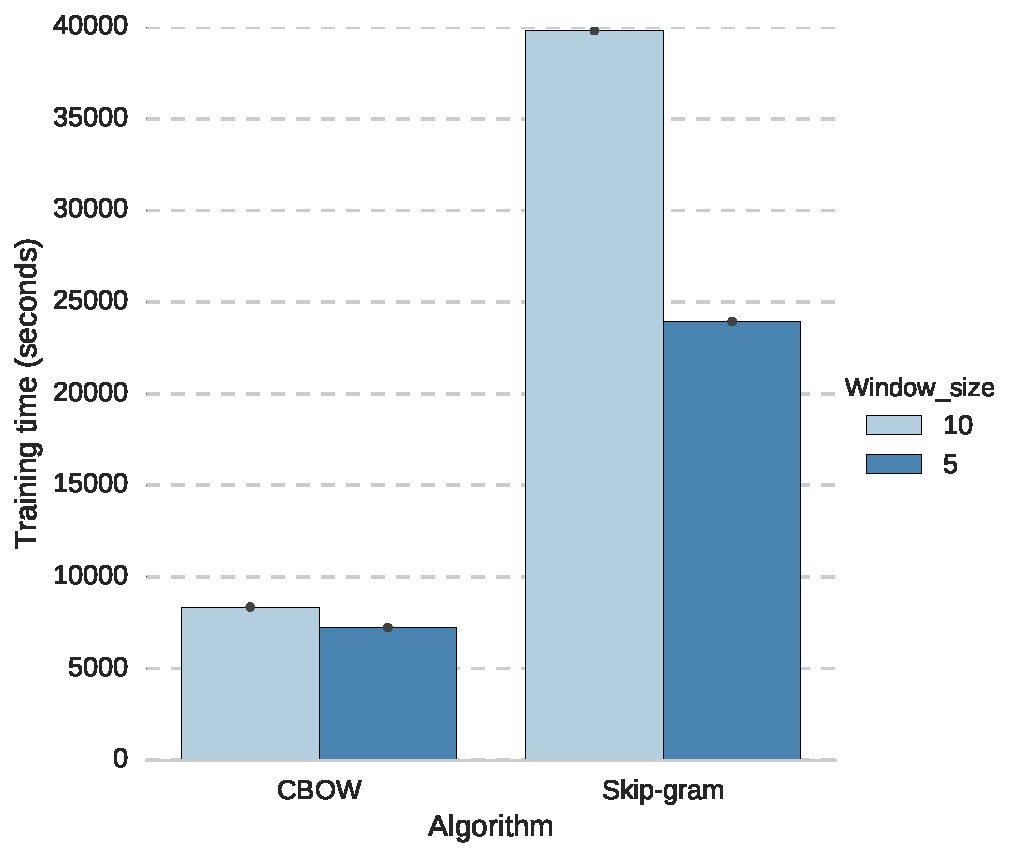
\includegraphics[width=0.9\textwidth]{./Figures/TrainTime-Window_size.pdf}
		\caption{}
		\label{fig:ds}
	\end{subfigure}\\
	\begin{subfigure}[b]{0.49\textwidth}
		\centering
		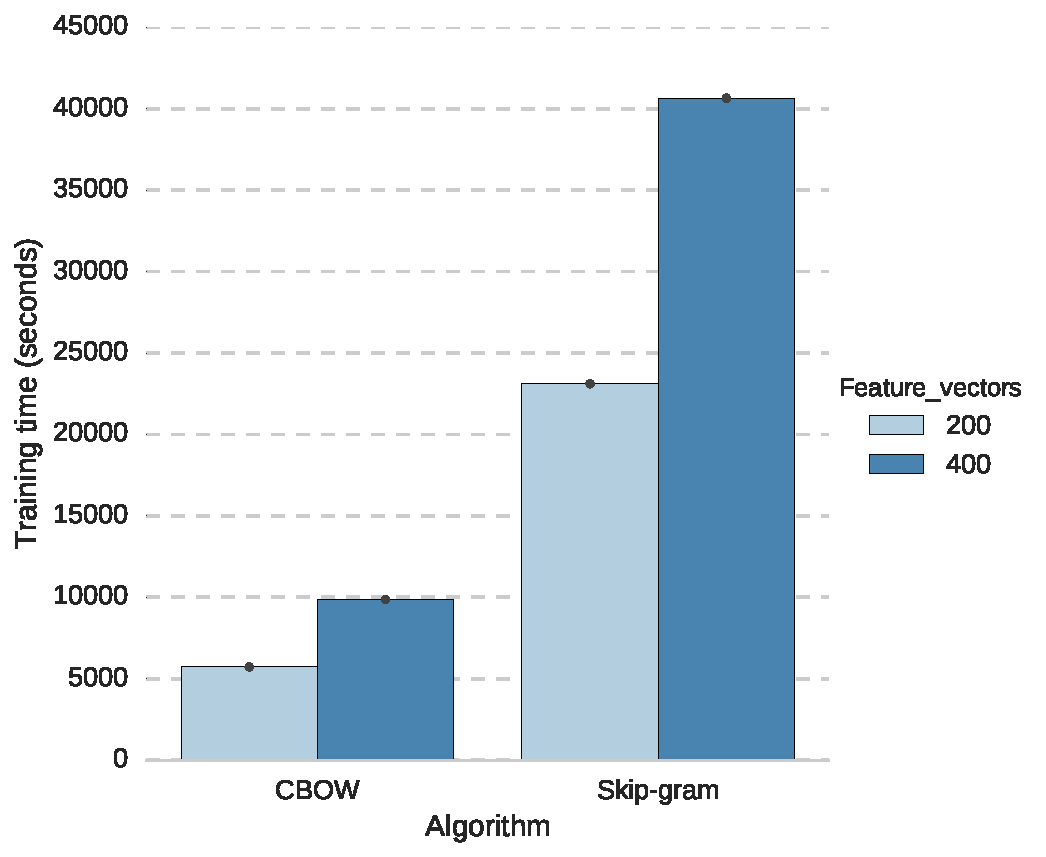
\includegraphics[width=0.9\textwidth]{./Figures/TrainTime-Feature_vectors.pdf}
		\caption{}
		\label{fig:fv}
	\end{subfigure}\\
	\caption*{Figure 2. Training time.}
	\label{fig:traintime}
\end{figure*}

\noindent\textbf{\emph{Concrete noun classification task.}} Here the task is to classify the set of given concrete nouns into two, three, and six clusters. Classification accuracy at each level is given in Table 3. Recall that the two clusters are representing "natural" and "artifact". Thus, the model was able to correctly classify  $97.7 \%$ of the concrete into "natural" and "artifact", whereas the classification into "animal", "vegetable", and "artifact" is correctly done for $95.5 \%$ of the words. 

\subsection*{5.2 Models trained on the Wikipedia English corpus}
As described in Section 4, two values are selected for each of the \emph{window size, down sampling, \emph{and} feature vectors (size)} parameters under both CBOW and Skip-gram. This results in 
$16$ different parameter combinations. Below, we discuss the performance of each of these.

\noindent\textbf{\emph{Training time.}} Figure 2 illustrates the training times pivoted around 
the architecture (CBOW or Skip-gram). The Skip-gram models (irrespective of the other parameter 
values) roughly took four times longer training time. When it comes to the parameters, window 
size (Figure 2b) and feature vectors (Figure 2c) appear to have larger impact on training time 
than down sampling(Figure 2a).

\noindent\textbf{\emph{Nearest neighbors.}} The large number of models makes it difficult to 
give a compact analysis of the nearest words data set. However, a random visual check was 
performed to verify the sanity of the trained models. CSV files containing the nearest words of all the words for all the models are available and can be shared upon request.
%Moreover, the top 5 nearest words of the first 40 words is given in Appendix A for the Skip-gram model with window size = 10, down sampling = 0.001 and feature vectors = 400.

\noindent\textbf{\emph{Analogical reasoning.}} The performance of all 16 models on the google analogical reasoning task is shown in Table 4. Looking at the \emph{currency} column, one can quickly see that all the models consistently gave very poor performance (an order of magnitude
poorer than the google embedding discussed in the previous section). Despite the significant 
amount of training time difference between the CBOW and Skip-gram models, they achieved equivalent performance in the analogical reasoning task, except for the \emph{capital-world} and \emph{city-in-state} sets, where the Skip-gram modes have a marginal edge over the CBOW.

\begin{figure}
	\centering
	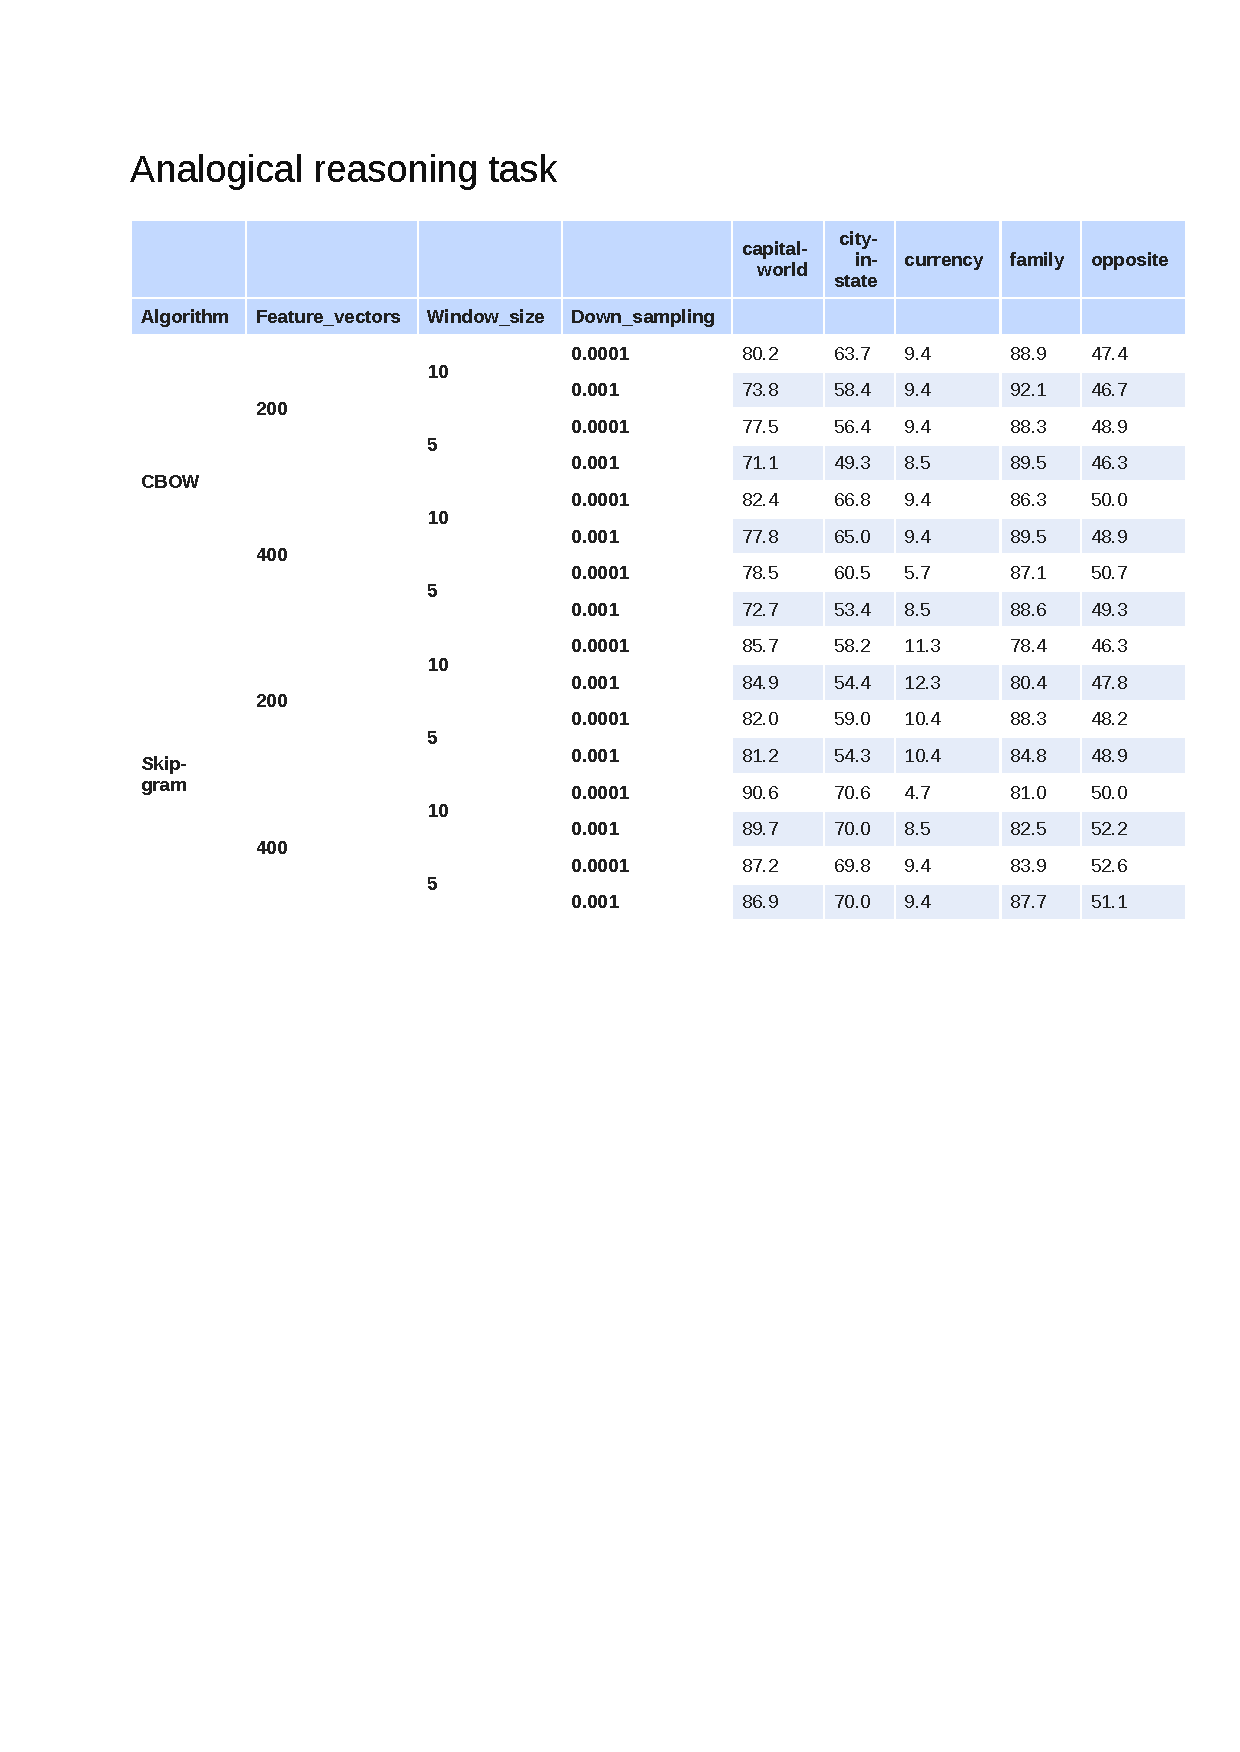
\includegraphics[trim=1cm 13cm 0cm 3.25cm, clip=true,width=\textwidth]{./Figures/summary-analogical.pdf}
	\caption*{Table 4. Accuracy (in $\%$) of analogical reasoning task result.}
	\label{fig:ana}
	
\end{figure}

\begin{figure}
	\centering
	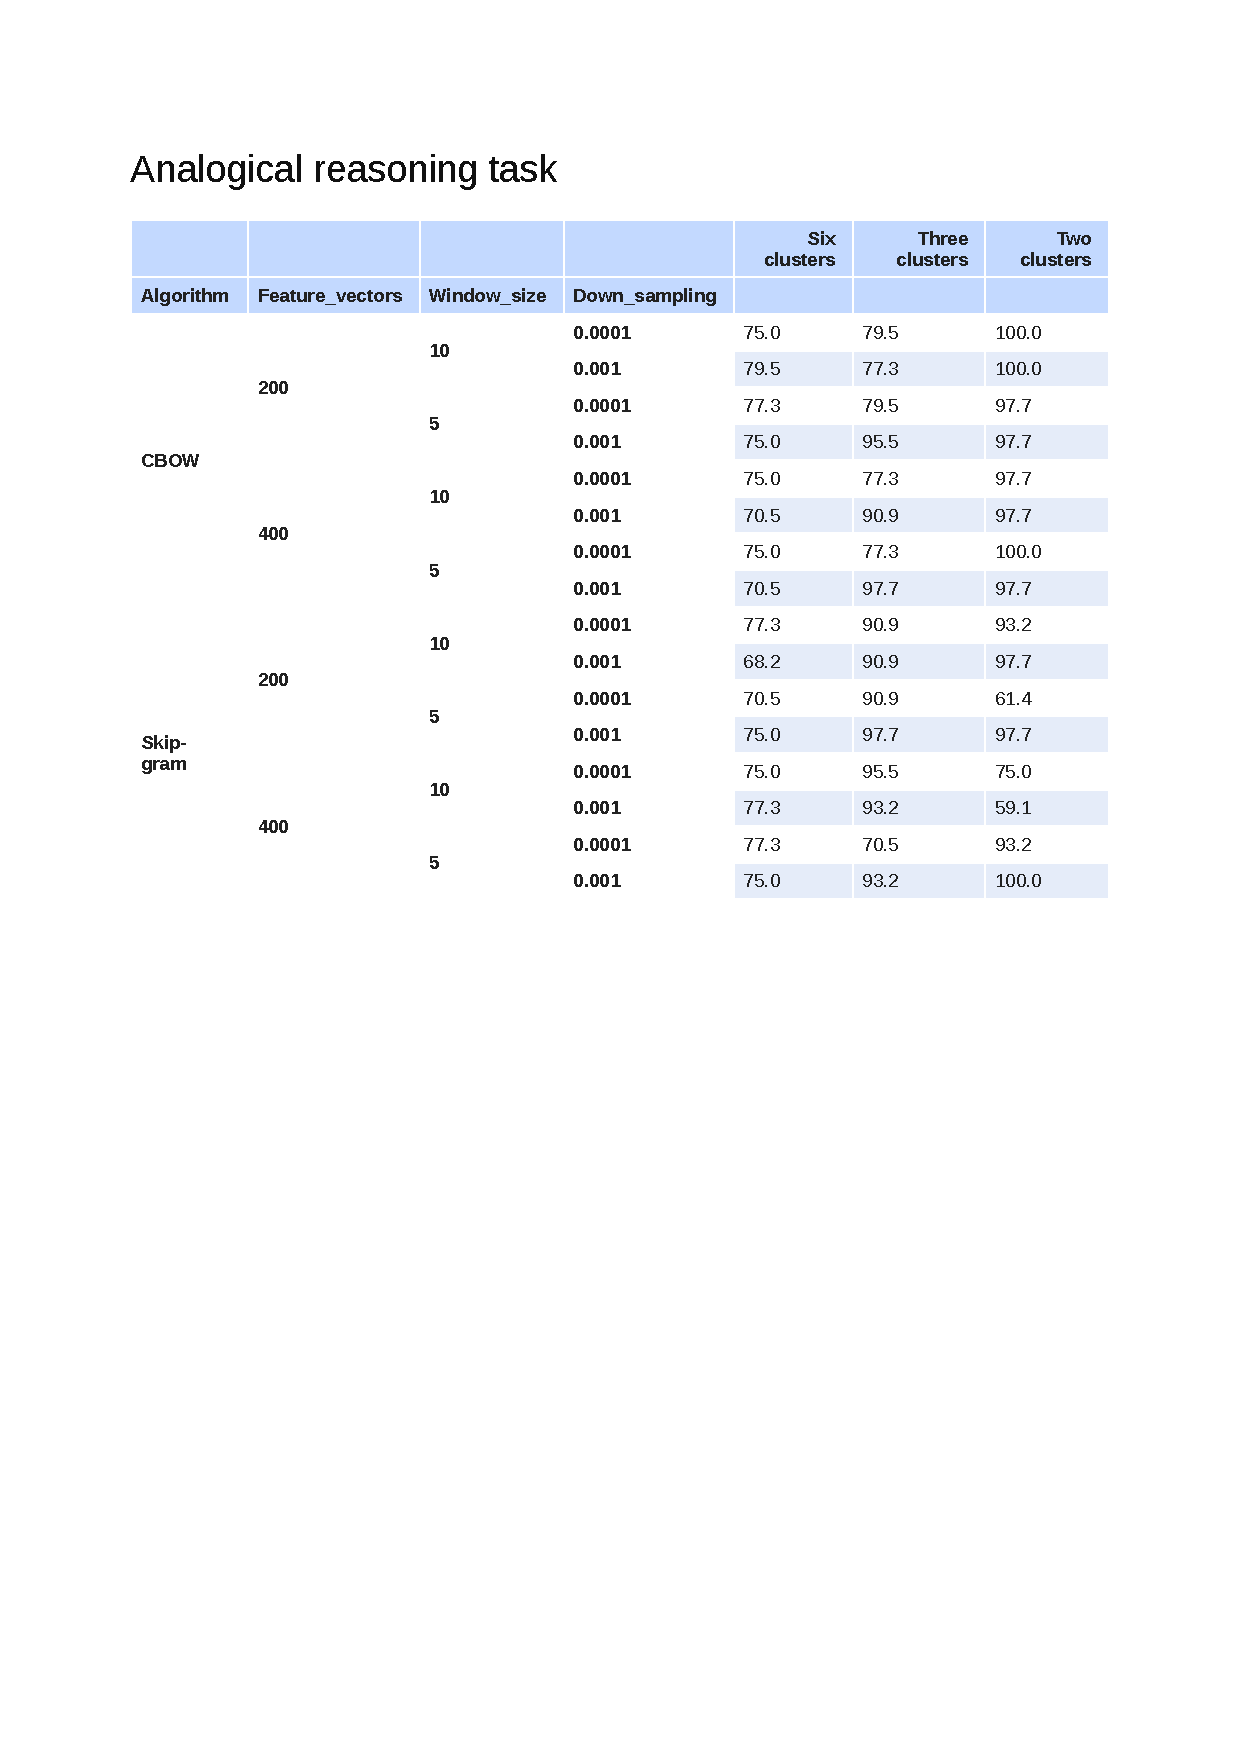
\includegraphics[trim=1cm 13cm 0cm 3.25cm, clip=true,width=\textwidth]{./Figures/summary-categorical.pdf}
	\caption*{Table 5. Concrete noun categorization task result.}
	\label{fig:cata}
	
\end{figure}
\noindent\textbf{\emph{Concrete noun categorization.}} Table 5 shows the performance of all the 
embeddings on three of the concrete noun categorization tasks. Once again, the CBOW and Skip-gram 
models gave comparable result. All the models gave impressive performance in classifying the nouns into two clusters, that is, "natural" and "artifact". The best of these models performed better than the google embedding on the two cluster task ($100\%$ accuracy), although the google embedding gave better performance on the six cluster task.

\section*{6. Conclusion}
In this project we conducted a comparative study of word embeddings trained using the Word2Vec
tool. In addition to training a number of models using the Wikipedia English corpus, we also  used publicly available embedding pre-trained using the Google news data set. Models are trained using both CBOW and Skip-gram. Different parameter values are also tested for window size, down sampling, and the size of feature vectors. The Skip-gram models roughly took four times longer training time than the CBOW models. However, the Skip-gram models did not perform any better than the CBOW models in the analogical reasoning and concrete noun categorization evaluation tasks.
%-------------------------------------------------------------------------------
% REFERENCES
%-------------------------------------------------------------------------------
\newpage
%\section*{References}
%\addcontentsline{toc}{section}{References}
\bibliographystyle{ieeetran}
\bibliography{reference.bib}

%Anand, U., 2010. The Elusive Free Radicals, \textit{The Clinical Chemist,} [e-journal] %Available at:<\url{http://www.clinchem.org/content/56/10/1649.full.pdf}> [Accessed 2 November 2013]
%\newline
%\newline

%Biology Forums, 2012. \textit{Normal glomerulus. Acute glomerulonephritis.} [online] Available at: <\url{http://biology-forums.com/index.php?action=gallery;sa=view;id=9284}> [Accessed 23 October 2013].
%\newline
%\newline
\newpage
\section*{Appendix}
\subsection*{A. Packages}
Python is used for programming tasks of this project. In addition to the standard library, the
following packages are used:

\begin{itemize}
	\item[1.] Matplotlib and Seaborn: For plotting
	\item[2.] Pandas: For reading evaluation sets and manipulating results.
	\item[3.] Numpy: For numerical calculations
	\item[4.] Sklean: for K-means clustering
\end{itemize}

\newpage
\subsection*{B. Code for training model}

\begin{lstlisting}
from gensim.models import word2vec
import os
import logging
logging.basicConfig(format='%(asctime)s : %(levelname)s : %(message)s',level=logging.INFO)

'''The corpus class is borrowed from https://rare-technologies.com/word2vec-tutorial/'''
class Corpus(object):
	def __init__(self, fname):
		self.fname = fname

	def __iter__(self):
		for line in open(self.fname):
			yield line.split()



def trainModel(Arch, windowSize, downSampling, numFeatures):
	file = os.path.join(os.getcwd(),'Term-project/Data/wikipedia2008_en.txt')
	sentences = Corpus(file) # a memory-friendly iterator
	if Arch == 0:
		alg = 'CBOW'
	else:
		alg = 'SkipGram'

	print('Training model with parameters: ')
	print('\tArchitecture {}'.format(alg))
	print('\tWindow size {}'.format(windowSize))
	print('\tDown sampling {}'.format(downSampling))
	print('\tNumber of feature vectors {} \n'.format(numFeatures))

	model = word2vec.Word2Vec(sentences, sg=Arch, window = windowSize, \
	   sample=downSampling, size=numFeatures, min_count = 20, workers=4)

	model.init_sims(replace=True)

	model_name = alg+'_ws'+ str(windowSize) + '_ds'+ str(downSampling) + '_ft' + str(numFeatures)
	model.save(model_name)
	model = None
	sentences = None
	
	
arch = [0,1] 
ws = [5,10]
ds = [0.001,0.0001]
fv = [200, 400]

with open("performanceLog.txt", 'a') as f:
	f.write("Architecture,Window Size, Down Sampling, Feature Vector, Start  Time, End Time\n")


for arch_item in arch:
	for ws_item in ws:
		for ds_item in ds:
			for fv_item in fv:

				if arch_item == 0:
					alg = "CBOW"
				else :
					alg = "SkipGram"
				start = str(datetime.now()) 

				trainModel(arch_item, ws_item, ds_item, fv_item)       

				end = str(datetime.now())

				with open("performanceLog.txt", 'a') as f:
				f.write(alg+","+str(ws_item)+","+str(ds_item)+","+str(fv_item)+","+start+","+end+"\n")	
\end{lstlisting}

\newpage
\subsection*{C. Code for trained model evaluation}
\begin{lstlisting}
import numpy as np
import gensim
import pandas as pd
from datetime import datetime
from sklearn.cluster import KMeans

'''An object of the class "Model" is a trained model
that is ready to be evaluated on the evaluation sets'''
class Model():
	def __init__(self, name, google=False):
		self.name = name
		self.analogical = []
		self.noun_classification = {}
		if google:
			self.model = gensim.models.Word2Vec.load_word2vec_format(name,binary=True)
		else:
			self.model = gensim.models.word2vec.Word2Vec.load(name)
			self.train_time = self.model.total_train_time

	def eval_nearest(self, target_words):
		self.nearest_words = pd.DataFrame(columns=["First","Second","Third","Fourth","Fifth"],index=target_words)

		for word in target_words:
		try:
			similar_words = self.model.most_similar(word, topn=5)
		except:
			continue
		for i in range(len(similar_words)):
			self.nearest_words.ix[word,i] = similar_words[i][0]

	def eval_analogical(self, file):
		self.accuracy = self.model.wv.accuracy(file)
		for i in range(len(self.accuracy)):
			self.analogical.append(round(100*len(self.accuracy[i]["correct"])/(len(self.accuracy[i]["correct"])+len(self.accuracy[i]["incorrect"])),1))
		label = ['capital-world','currency','city-in-state','family','opposite']
		self.analogical = dict(zip(label, self.analogical))

	def conc_noun_kmeans(self,word_list):
		self.word_vec = np.zeros([len(word_list), len(self.model.wv.syn0[0])])
		self.word_cluster = pd.DataFrame(word_list,columns=["Words"])
		for i in range(len(word_list)):
			self.word_vec[i] = self.model[word_list[i]]
		for c in [2,3,6]: 
			self.kmeans_clustering = KMeans(n_clusters = c)
			self.cluster = self.kmeans_clustering.fit_predict(self.word_vec)
			self.word_cluster["Clusters_"+str(c)] = self.cluster

	def eval_classification(self, concrete_nouns):
		bi_cluster = [self.word_cluster[self.word_cluster["Clusters_2"] == i]["Words"].tolist() for i in [0,1]]
		tri_cluster = [self.word_cluster[self.word_cluster["Clusters_3"] == i]["Words"].tolist() for i in [0,1,2]]
		hex_cluster = [self.word_cluster[self.word_cluster["Clusters_6"] == i]["Words"].tolist() for i in range(6)]

		self.bi_class_error(bi_cluster, concrete_nouns)
		self.tri_class_error(tri_cluster, concrete_nouns)
		self.hex_class_error(hex_cluster, concrete_nouns)

	def bi_class_error(self, cluster_of_words, concrete_nouns):
		error = []
		for i in range(len(cluster_of_words)):
		cluster = {'natural': 0, 'artifact': 0}
		tmp = concrete_nouns.set_index("Words")

		for word in cluster_of_words[i]:
			if tmp.loc[word, "fClusters_2"] == "natural":
				cluster['natural'] += 1
			elif tmp.loc[word, "fClusters_2"] == "artifact":
				cluster['artifact'] += 1

		count = [ item for item in list(cluster.values()) if item != 0 ]

		if len(count) == 1:
			error.append(0.0)
			continue
		elif len(count) > 1:
			count = sorted(count, reverse=True)
			count.pop(0)
			for val in count:
				error.append(val)

		self.noun_classification["two_class_classification"] = 100 - round(100*sum(error)/concrete_nouns.Words.size, 1)

	def tri_class_error(self, cluster_of_words, concrete_nouns):
		error = []
		for i in range(len(cluster_of_words)):
			cluster = {'animal': 0, 'vegetable': 0, 'artifact': 0}
			tmp = concrete_nouns.set_index("Words")

			for word in cluster_of_words[i]:
				if tmp.loc[word, "fClusters_3"] == "animal":
					cluster['animal'] += 1
				elif tmp.loc[word, "fClusters_3"] == "vegetable":
					cluster['vegetable'] += 1
				elif tmp.loc[word, "fClusters_3"] == "artifact":
					cluster['artifact'] += 1
			count = [ item for item in list(cluster.values()) if item != 0 ]

			if len(count) == 1:
				error.append(0.0)
				continue
			elif len(count) > 1:
				count = sorted(count, reverse=True)
				count.pop(0)
				for val in count:
					error.append(val)
		self.noun_classification["three_class_classification"] = 100 - round(100*sum(error)/concrete_nouns.Words.size, 1)

	def hex_class_error(self, cluster_of_words, concrete_nouns):
		error = []
		for i in range(len(cluster_of_words)):
			cluster = {'bird': 0,'groundAnimal': 0, 'fruitTree': 0, 'green': 0, 'tool': 0, 'vehicle': 0}
			tmp = concrete_nouns.set_index("Words")

			for word in cluster_of_words[i]:
				if tmp.loc[word, "fClusters_6"] == "bird":
					cluster['bird'] += 1
				elif tmp.loc[word, "fClusters_6"] == "groundAnimal":
					cluster['groundAnimal'] += 1
				elif tmp.loc[word, "fClusters_6"] == "fruitTree":
					cluster['fruitTree'] += 1
				elif tmp.loc[word, "fClusters_6"] == "green":
					cluster['green'] += 1
				elif tmp.loc[word, "fClusters_6"] == "tool":
					cluster['tool'] += 1
				elif tmp.loc[word, "fClusters_6"] == "vehicle":
					cluster['vehicle'] += 1
			count = [ item for item in list(cluster.values()) if item != 0 ]

			if len(count) == 1:
				error.append(0.0)
					continue
			elif len(count) > 1:
				count = sorted(count, reverse=True)
				count.pop(0)
				for val in count:
					error.append(val)

		self.noun_classification["six_class_classification"] = 100 - round(100*sum(error)/concrete_nouns.Words.size, 1)



def read_conc_nouns():
	cluster = pd.read_csv("Data/eval/ESSLLI2008_concNouns.categorization.dataset_en.txt", sep="\t",usecols=["NOUN","CLASS"])
	tmp = cluster.CLASS.apply(lambda x: x.split("-"))
	df = []
	for item in tmp:
	df.append(dict(zip("fClusters_6 fClusters_3 fClusters_2".split(),item)))
	df = pd.DataFrame(df)

	cluster.drop("CLASS",axis=1,inplace=True)
	cluster.rename(columns={"NOUN":"Words"},inplace=True)
	cluster = cluster.join(df)

	return cluster

def load_and_evaluate(modelName, google=False): 
	model = Model(modelName, google)

	# Evaluate nearest words
	print("Starting nearest neighbor evaluation task...\n")
	nearest_file = "Data/eval/nearest_neighbor_wordlist.csv"
	eval_nearest = pd.read_csv(nearest_file,header=None,usecols=[1])
	target_words = eval_nearest.loc[:,1].values.tolist()

	model.eval_nearest(target_words)

	# Evaluate analogical reasoning task
	print("Starting analogical reasoning evaluation task...\n")
	model.eval_analogical("Data/eval/analogical_reasoning_questions-words-short.txt")


	# Evaluate concrete noun classification task
	print("Starting concrete noun categorization task...\n")
	concrete_nouns = read_conc_nouns()
	word_list = concrete_nouns.Words.tolist()
	model.conc_noun_kmeans(word_list)
	model.eval_classification(concrete_nouns)

	return model
	
def eval_google():
	df_final = pd.DataFrame()
	model_name = 'GoogleNews-vectors-negative300.bin.gz'
	m = model.load_and_evaluate(model_name, google=True) 
	df = pd.DataFrame([m.analogical])
	df = df.join(pd.DataFrame([m.noun_classification]))

	df_final = df_final.append(df,ignore_index=True)
	df_final.to_csv(os.getcwd()+"/results/google-evaluation_result.csv")
	m.nearest_words.to_csv(os.getcwd()+"/results/google-nearest_words.csv")
	
def eval_wikipedia():	
	arch = [0,1] 
	ws = [5, 10] 
	ds = [0.001,0.0001]
	fv = [200, 400]

	df_final = pd.DataFrame()

	for arch_item in arch:
		for ws_item in ws:
			for ds_item in ds:
				for fv_item in fv:

					if arch_item == 0:
						alg = "CBOW"
					else :
						alg = "SkipGram"
					model_name = alg+'_ws'+ str(ws_item) + '_ds'+ str(ds_item) + '_ft' + str(fv_item)
					m = model.load_and_evaluate(model_name) 
					df = pd.DataFrame([m.analogical])
					df = df.join(pd.DataFrame([m.noun_classification]))

					time = {"Train_time": m.train_time}
					df = df.join(pd.DataFrame([time]))
					df_final = df_final.append(df,ignore_index=True)
					df_final.to_csv(os.getcwd()+"/results/Evaluation_result.csv")
					m.nearest_words.to_csv(os.getcwd()+"/results/"+model_name+".csv")




\end{lstlisting}

\end{document}

